%!TEX root = ../tudkom_students__201804_v1.4.tex
\chapter{Evaluation}
\label{ch:evaluation}
%This chapter should describe how the evaluation of the implemented mechanism was done.
%1. Which evaluation method is used and why? Simulations, prototype?
%2. What is the goal of the evaluation? Comparison? Proof of concept?
%3. Wich metrics are used for characterizing the performance, costs, fairness, and efficiency of the system?
%4. What are the parameter settings used in the evaluation and why? If possible always justify why a certain threshold has been chose for a particular parameter.
%5. What is the outcome of the evaluation?
% 5-10 pages

\section{Ziele}
\label{ch:aimEval}
Mit dem Wearable werden einige Tests mit Blick auf die in der Einleitung \ref{ch:aims} aufgestellten Ziele gemacht.
Die Austauschbarkeit der Protokolle und Komponenten wird durch die Implementierung erreicht.
Insbesondere die Trennung des Codes von Endgerät, MCU, IMU und dem Protokoll zwischen MCU und IMU tragen dazu bei.
Ob die Größe und das Gewicht ausreichend gering sind, ist vom Anwendungsfall abhängig.
Bei dem Wearable sind sie stark von der Knopfzelle geprägt.
Es wurde die etwa 2.36 cm\textsuperscript{3} große CR2450 statt der etwa 1.01 cm\textsuperscript{3} großen CR2032 gewählt um die 2.7-fache Kapazität zu erhalten.
Um die Entscheidung zu ändern, muss nur das Platinenlayout überarbeitet werden während das Schaltbild und der Code übernommen werden können.
Ob die Kapazität der Knopfzellen überhaupt anwendungstauglich ist, soll in den Tests zur Stromaufnahme ermittelt werden.
Dafür sollen verschiedene Parameter geändert werden und der Einfluss auf die Stromaufnahme gemessen und die Auswirkungen auf die Datenübertragung evaluiert werden.
Bei der Datenübertragung kann zum Einen die Menge der Sensordaten pro Sekunde gemessen werden.
Zum Anderen kann geprüft werden, wie regelmäßig die Sensordaten beim Endgerät ankommen.\\
Es wurde die Stromaufnahme verglichen in den Szenarien Prototyp mit LSM6DSL IMU vs Wearable und LSM6DSL IMU vs BMI160 IMU auf dem Prototypen.
Der Prototyp besteht aus dem nRF52 DK und dem STEVAL-MKI178V2 bzw. BMI160 Shuttle Board.
Die Auswirkungen auf die Stromaufnahme und der Datenübertragung werden auf dem Wearable bei einer Änderung der Größe des TX-Buffers, der MTU-Größe, dem Connection Interval, der SPI-Frequenz und der Sensordatenrate erfasst.
Um den Einfluss des Algorithmus zu erfassen, werden die Test mit der variablen Größe des TX-Buffers auch ohne aktivem Algorithmus getestet.
Dafür wird dem Algorithmus eine Größe des TX-Buffers von 0xFFFFu in \texttt{main.c} in der Zeile \texttt{err\_code = my\_service\_init(\allowbreak{}\&m\_myservice, TX\_QUEUE\_SIZE);} übergeben.

\section{Methoden}
Zur Messung der Datenrate wird auf dem Smartphone angezeigt, wie viele Datenpakete in einer Sekunde ankommen.
Um die Regelmäßigkeit zu vergleichen wird die Datenrate pro Sekunde über einen Zeitraum aufgenommen und die Formel \ref{eq:standardabweichung} für die Standardabweichung mit dem unverzerrten Schätzer angewandt.
\begin{equation}
  \label{eq:standardabweichung}
	s = \sqrt{\cfrac{1}{n-1}\sum_{i=1}^{n} (x_{i}-\overline{x})^{2}}\text{, mit n = Anzahl der Werte und $\overline{x}$ = eingestellte Sensordatenrate}
\end{equation}
Die Standardabweichung wird wiederum in einem anderem Graphen auf dem Smartphone aufgezeichnet, sobald Daten von mindestens 30 Sekunden vorliegen.\\
Um die Stromaufnahme zu messen, wird das ohmsche Gesetz $I = \cfrac{U}{R}$ benötigt.
Wird ein Widerstand in Reihe mit der Spannungsversorgung des Wearables geschaltet, ist ein Spannungsabfall um den Widerstand zu messen.
Da man den Wert des Widerstandes kennt und den Spannungsabfall mit einem Oszilloskop messen kann, lässt sich mit der Formel der Strom berechnen.
Bei der Wahl des Widerstandes gilt: Je größer der Widerstand, desto mehr Spannung fällt ab.
Ist die Spannung zu klein, lässt sie sich nicht genau messen.
Ist die Spannung zu groß, bleibt nicht genug Spannung für das Wearable übrig.
Um den Strom in verschiedenen Messbereichen berechnen zu können, werden die passenden Widerstände benötigt.
Um den Widerstand anpassen zu können, wurde eine Lochrasterplatine, die in Abbildung \ref{fig:messplatine} zu sehen ist, mit Widerständen bestückt, die mit Steckbrücken in den Stromkreis integriert werden können.
\begin{figure}[hbtp]
	\centering
	\includegraphics[width=0.45\linewidth]{res/messplatine.jpg}
	\caption{Messplatine}
	\label{fig:messplatine}
\end{figure}
Die Widerstände haben eine Toleranz von 0.1 \% und Werte von 0, 10, 47, 100, 470, 1000, 4700 und 10000 Ohm.\\
Das Oszilloskop ist ein Picoscope 5444B.
Der Spannungsabfall wurde mit einer Frequenz 2 GHz gemessen.
Technisch bedingt kann der Mittelwert nur über 5 Sekunden automatisch gebildet werden.
Deshalb wurde jeder Test 6 Mal abgeschlossen.
Das Offset wurde vor dem Test kalibriert.
Als Spannungsquelle wurde eine neue CR2450 Knopfzelle und ein Voltcraft Model 2256 Netzgerät genutzt.
Da das Netzteil bei zu geringer Last oder bei einer schnellen großen Laständerung keine stabile Spannung erzeugen kann, wurde dem Testobjekt ein Widerstand von 58.75 Ohm +/- 5 \% parallel geschaltet.
Durch den Widerstand fließt dauerhaft etwa 51 mA, sodass das Netzteil mindestens eine Last von 3.4 \% hat.
Da das immer noch wenig ist, toleriert das Netzteil bei den Messungen einen geringeren Spannungsabfall bei den Messwiderständen als die Batterie.
Das Netzteil wurde so eingestellt, dass am Testobjekt eine Spannung zwischen 2.95 und 3 V anliegt.
Es wurde das Netzteil bei den Tests genutzt, bei denen der Prototyp involviert war, da er sich zum Testzeitpunkt aus unbekannten Gründen nicht mit der Batterie starten ließ.
Zu einem späteren Zeitpunkt war es wieder möglich.
Vor jeder Testreihe wurde die Spannung am Netzteil nachjustiert oder die Spannung der Batterie notiert.\\
Beim Prototypen wurde die Diode zum Verpolungsschutz mit SB12 überbrückt, wie in der Anleitung zum nRF52 DK angegeben \cite{site_nrf52dk}.
Der Spannungsabfall wurde direkt an der Spannungsquelle gemessen und nicht an den Pins 'nRF current measurement'.
Nach dem Schaltbild von Figur 8 in \cite{site_nrf52dk} ließe sich sonst nur der Strom, der von der MCU aufgenommen wird, messen und der Verbrauch der IMU wäre nicht mit eingegangen.
Der Hinweis über Figur 8 besagt, dass die MCU bei der verwendeten Methode wegen der Reset-Funktion 20 $\mu$A mehr Strom verbraucht.
Da der Reset-Knopf erst eine Funktion zeigt, wenn auch SB10 überbrückt wird, kann erst mit den vorliegenden Ergebnissen eine Aussage getroffen werden, ob sich der Prototyp dahingehend vom Wearable unterschiedet.
Der Magnetometer wurde beim BMI160 Shuttle Board nicht entfernt oder konfiguriert.

\section{Ergebnisse}
Der erste Teil der Tabellen listet die Rahmenbedingungen für die Tests auf.
Die Zeilen der Daten beginnen mit der Beschreibung des Testfalls.
Die Zeile 'AVG' ist der Durchschnitt der sechs Einzeltests.
Sie besteht aus gemessenem Spannungsabfall, der berechneten Stromaufnahme.
Die Zeile 'P\textsubscript{AVG}' ist die Leistungsaufnahme nach $P_{AVG} = (Versorgungsspannung - gemesseneSpannung) * resultierender Strom$.
Einzelne Tests haben zusätzlich die Standardabweichung 'ABW' oder listen die höchsten gemessenen Spitze im Spannungsabfall auf.

\begin{figure}[!hbtp]
  \begin{minipage}{0.5\textwidth}
    \centering
    \begin{tabular}{|l|l|l|}
      \hline
      Widerstand & \multicolumn{2}{l|}{10 Ohm}\\
      SPI-Frequenz & \multicolumn{2}{l|}{4 MHz}\\
      MTU-Größe & \multicolumn{2}{l|}{23 Byte}\\
      TX-Buffer & \multicolumn{2}{l|}{10 Einträge}\\
      Spannungsquelle & \multicolumn{2}{l|}{Netzteil}\\
      MCU & \multicolumn{2}{l|}{Wearable und Prototyp}\\
      IMU & \multicolumn{2}{l|}{LSM6DSL und BMI160}\\
      Sensordatenrate & \multicolumn{2}{l|}{200 Hz und 0 Hz}\\
      Connection Interval & \multicolumn{2}{l|}{High}\\
      \hline
      \multicolumn{3}{|c|}{Wearable LSM6DSL 200 Hz}\\
      AVG & 24.555 mV & 2.456 mA\\
      P\textsubscript{AVG} & \multicolumn{2}{c|}{7.246 mW}\\
      \hline
      \multicolumn{3}{|c|}{Wearable LSM6DSL 0 Hz}\\
      AVG & 3.55 mV & 355 $\mu$A\\
      P\textsubscript{AVG} & \multicolumn{2}{c|}{0.995 mW}\\
      \hline
      \multicolumn{3}{|c|}{Prototyp LSM6DSL 200 Hz}\\
      AVG & 29.455 mV & 2.946 mA\\
      P\textsubscript{AVG} & \multicolumn{2}{c|}{8.678 mW}\\
      \hline
      \multicolumn{3}{|c|}{Prototyp LSM6DSL 0 Hz}\\
      AVG & 10.153 mV & 1.015 mA\\
      P\textsubscript{AVG} & \multicolumn{2}{c|}{3.001 mW}\\
      \hline
      \multicolumn{3}{|c|}{Prototyp BMI160 200 Hz}\\
      AVG & 34.958 mV & 3.496 mA\\
      P\textsubscript{AVG} & \multicolumn{2}{c|}{10.278 mW}\\
      \hline
      \multicolumn{3}{|c|}{Prototyp BMI160 0 Hz}\\
      AVG & 10.031 mV & 1.003 mA\\
      P\textsubscript{AVG} & \multicolumn{2}{c|}{2.974 mW}\\
      \hline
    \end{tabular}
    \captionof{table}{Prototyp vs Wearable und BMI160 vs LSM6DSL}%
    \label{tab:test1}
  \end{minipage}
  \begin{minipage}{0.5\textwidth}
    \centering
    \begin{tabular}{|l|l|l|}
      \hline
      Widerstand & \multicolumn{2}{l|}{47 Ohm}\\
      SPI-Frequenz & \multicolumn{2}{l|}{1 MHz}\\
      MTU-Größe & \multicolumn{2}{l|}{23, 50 und 517 Byte}\\
      TX-Buffer & \multicolumn{2}{l|}{1, 50 und 300 Einträge}\\
      Algorithmus & \multicolumn{2}{l|}{An und Aus}\\
      Spannungsquelle & \multicolumn{2}{l|}{Batterie 3.044 V}\\
      MCU & \multicolumn{2}{l|}{Wearable}\\
      IMU & \multicolumn{2}{l|}{LSM6DSL}\\
      Sensordatenrate & \multicolumn{2}{l|}{200 Hz}\\
      Connection Interval & \multicolumn{2}{l|}{High}\\
      \hline
      \multicolumn{3}{|c|}{MTU23 TX1 Algo=An}\\
      AVG & 125.267 mV & 2.665 mA\\
      P\textsubscript{AVG} & \multicolumn{2}{c|}{7.778 mW}\\
      ABW & \multicolumn{2}{c|}{10.4 - 10.8 Hz}\\
      \hline
      \multicolumn{3}{|c|}{MTU23 TX50 Algo=An}\\
      AVG & 126.2 mV & 2.685 mA\\
      P\textsubscript{AVG} & \multicolumn{2}{c|}{7.834 mW}\\
      ABW & \multicolumn{2}{c|}{10.2 - 11.5 Hz}\\
      \hline
      \multicolumn{3}{|c|}{MTU23 TX300 Algo=An}\\
      AVG & 126.217 mV & 2.664 mA\\
      P\textsubscript{AVG} & \multicolumn{2}{c|}{7.773 mW}\\
      ABW & \multicolumn{2}{c|}{8.2 - 8.8 Hz}\\
      \hline
      \multicolumn{3}{|c|}{MTU23 TX1 Algo=Aus}\\
      AVG & 125.317 mV & 2.666 mA\\
      P\textsubscript{AVG} & \multicolumn{2}{c|}{7.781 mW}\\
      ABW & \multicolumn{2}{c|}{11.9 - 12.4 Hz}\\
      \hline
      \multicolumn{3}{|c|}{MTU23 TX50 Algo=Aus}\\
      AVG & 125.883 mV & 2.678 mA\\
      P\textsubscript{AVG} & \multicolumn{2}{c|}{7.815 mW}\\
      ABW & \multicolumn{2}{c|}{12 - 12.7 Hz}\\
      \hline
      \multicolumn{3}{|c|}{MTU23 TX300 Algo=Aus}\\
      AVG & 125.9 mV & 2.679 mA\\
      P\textsubscript{AVG} & \multicolumn{2}{c|}{7.818 mW}\\
      ABW & \multicolumn{2}{c|}{12 - 13.2 Hz}\\
      \hline
    \end{tabular}
    \captionof{table}{Größenänderung von TX-Buffer und MTU}%
    \label{tab:test2}
  \end{minipage}
\end{figure}

\begin{figure}[!hbtp]
  \begin{minipage}{0.5\textwidth}
    \centering
    \begin{tabular}{|l|l|l|}
      \hline
      \multicolumn{3}{|c|}{MTU150 TX10 Algo=An}\\
      AVG & 125.8 mV & 2.677 mA\\
      P\textsubscript{AVG} & \multicolumn{2}{c|}{7.812 mW}\\
      ABW & \multicolumn{2}{c|}{8.9 - 10.1 Hz}\\
      \hline
      \multicolumn{3}{|c|}{MTU517 TX10 Algo=An}\\
      AVG & 126.1 mV & 2.683 mA\\
      P\textsubscript{AVG} & \multicolumn{2}{c|}{7.829 mW}\\
      ABW & \multicolumn{2}{c|}{8.4 - 9.4 Hz}\\
      \hline
      \multicolumn{3}{|c|}{MTU150 TX50 Algo=An}\\
      AVG & 125.783 mV & 2.676 mA\\
      P\textsubscript{AVG} & \multicolumn{2}{c|}{7.809 mW}\\
      ABW & \multicolumn{2}{c|}{10.3 - 11.2 Hz}\\
      \hline
    \end{tabular}
    \captionof{table}{Fortsetzung von Tabelle \ref{tab:test2}}%
    \label{tab:test2b}
    \hfill \break
    \hfill \break
    \begin{tabular}{|l|l|l|}
      \hline
      Widerstand & \multicolumn{2}{l|}{47 Ohm}\\
      SPI-Frequenz & \multicolumn{2}{l|}{125 kHz, 1 MHz, 8 MHz}\\
      MTU-Größe & \multicolumn{2}{l|}{35 Byte}\\
      TX-Buffer & \multicolumn{2}{l|}{10 Einträge}\\
      Spannungsquelle & \multicolumn{2}{l|}{Batterie 3.044 V}\\
      MCU & \multicolumn{2}{l|}{Wearable}\\
      IMU & \multicolumn{2}{l|}{LSM6DSL}\\
      Sensordatenrate & \multicolumn{2}{l|}{400 Hz}\\
      Connection Interval & \multicolumn{2}{l|}{High}\\
      \hline
      \multicolumn{3}{|c|}{125kHz}\\
      AVG & 294.95 mV & 6.276 mA\\
      P\textsubscript{AVG} & \multicolumn{2}{c|}{17.253 mW}\\
      ABW & \multicolumn{2}{c|}{21.4 - 23 Hz}\\
      \hline
      \multicolumn{3}{|c|}{1MHz}\\
      AVG & 187.817 mV & 3.996 mA\\
      P\textsubscript{AVG} & \multicolumn{2}{c|}{11.413 mW}\\
      ABW & \multicolumn{2}{c|}{15.7 - 17.8 Hz}\\
      \hline
      \multicolumn{3}{|c|}{8MHz}\\
      AVG & 173.233 mV & 3.686 mA\\
      P\textsubscript{AVG} & \multicolumn{2}{c|}{10.582 mW}\\
      ABW & \multicolumn{2}{c|}{15.1 - 17.1 Hz}\\
      \hline
    \end{tabular}
    \captionof{table}{Frequenzänderung von SPI}%
    \label{tab:test3}
  \end{minipage}
  \begin{minipage}{0.5\textwidth}
    \centering
    \begin{tabular}{|l|l|l|}
      \hline
      Widerstand & \multicolumn{2}{l|}{47 Ohm}\\
      SPI-Frequenz & \multicolumn{2}{l|}{4 MHz}\\
      MTU-Größe & \multicolumn{2}{l|}{35 Byte}\\
      TX-Buffer & \multicolumn{2}{l|}{10 Einträge}\\
      Spannungsquelle & \multicolumn{2}{l|}{Batterie 2.991 V}\\
      MCU & \multicolumn{2}{l|}{Wearable}\\
      IMU & \multicolumn{2}{l|}{LSM6DSL}\\
      Sensordatenrate & \multicolumn{2}{l|}{0 und 100 Hz}\\
      Connection Interval & \multicolumn{2}{l|}{Low, Balance, High}\\
      \hline
      \multicolumn{3}{|c|}{Low 0Hz}\\
      AVG & 22.715 mV & 483.298 $\mu$A\\
      P\textsubscript{AVG} & \multicolumn{2}{c|}{1.435 mW}\\
      \hline
      \multicolumn{3}{|c|}{Balance 0Hz}\\
      AVG & 27.27 mV & 580.213 $\mu$A\\
      P\textsubscript{AVG} & \multicolumn{2}{c|}{1.72 mW}\\
      \hline
      \multicolumn{3}{|c|}{High 0Hz}\\
      AVG & 36.652 mV & 779.83 $\mu$A\\
      P\textsubscript{AVG} & \multicolumn{2}{c|}{2.304 mW}\\
      \hline
      \multicolumn{3}{|c|}{Low 100Hz}\\
      AVG & 83.443 mV & 1.775 mA\\
      P\textsubscript{AVG} & \multicolumn{2}{c|}{5.161
       mW}\\
       ABW & \multicolumn{2}{c|}{7.3 - 8.2 Hz}\\
      \hline
      \multicolumn{3}{|c|}{Balance 100Hz}\\
      AVG & 86.188 mV & 1.834 mA\\
      P\textsubscript{AVG} & \multicolumn{2}{c|}{5.327 mW}\\
      ABW & \multicolumn{2}{c|}{5.5 - 6.3 Hz}\\
      \hline
      \multicolumn{3}{|c|}{High 100Hz}\\
      AVG & 94.575 mV & 2.012 mA\\
      P\textsubscript{AVG} & \multicolumn{2}{c|}{5.828 mW}\\
      ABW & \multicolumn{2}{c|}{4.7 - 5.1 Hz}\\
      \hline
    \end{tabular}
    \captionof{table}{Änderung des Connection Interval}%
    \label{tab:test4}
  \end{minipage}
\end{figure}

\begin{figure}[!hbtp]
  \begin{minipage}{0.5\textwidth}
    \centering
    \begin{tabular}{|l|l|l|}
      \hline
      Widerstand & \multicolumn{2}{l|}{47 Ohm}\\
      SPI-Frequenz & \multicolumn{2}{l|}{4 MHz}\\
      MTU-Größe & \multicolumn{2}{l|}{35 Byte}\\
      TX-Buffer & \multicolumn{2}{l|}{10 Einträge}\\
      Spannungsquelle & \multicolumn{2}{l|}{Batterie 2.991 V}\\
      MCU & \multicolumn{2}{l|}{Wearable}\\
      IMU & \multicolumn{2}{l|}{LSM6DSL}\\
      Sensordatenrate & \multicolumn{2}{l|}{25 bis 800 Hz}\\
      Connection Interval & \multicolumn{2}{l|}{High}\\
      \hline
      \multicolumn{3}{|c|}{25Hz}\\
      AVG & 78.043 mV & 1.66 mA\\
      P\textsubscript{AVG} & \multicolumn{2}{c|}{4.836 mW}\\
      \hline
      \multicolumn{3}{|c|}{50Hz}\\
      AVG & 83.378 mV & 1.774 mA\\
      P\textsubscript{AVG} & \multicolumn{2}{c|}{5.158 mW}\\
      \hline
      \multicolumn{3}{|c|}{100Hz}\\
      AVG & 98.362 mV & 2.093 mA\\
      P\textsubscript{AVG} & \multicolumn{2}{c|}{6.054 mW}\\
      \hline
      \multicolumn{3}{|c|}{200Hz}\\
      AVG & 125.233 mV & 2.665 mA\\
      P\textsubscript{AVG} & \multicolumn{2}{c|}{7.637 mW}\\
      \hline
      \multicolumn{3}{|c|}{400Hz}\\
      AVG & 180.817 mV & 3.847 mA\\
      P\textsubscript{AVG} & \multicolumn{2}{c|}{10.811 mW}\\
      \hline
      \multicolumn{3}{|c|}{800Hz}\\
      AVG & 286.167 mV & 6.089 mA\\
      P\textsubscript{AVG} & \multicolumn{2}{c|}{16.47 mW}\\
      \hline
    \end{tabular}
    \captionof{table}{Änderung der Sensordatenrate}%
    \label{tab:test5}
  \end{minipage}
  \begin{minipage}{0.5\textwidth}
    \centering
    \begin{tabular}{|l|l|l|}
      \hline
      Widerstand & \multicolumn{2}{l|}{47 und 10000 Ohm}\\
      SPI-Frequenz & \multicolumn{2}{l|}{8 MHz}\\
      MTU-Größe & \multicolumn{2}{l|}{23 Byte}\\
      TX-Buffer & \multicolumn{2}{l|}{17 Einträge}\\
      Spannungsquelle & \multicolumn{2}{l|}{Batterie 2.875 und 2.916 V}\\
      MCU & \multicolumn{2}{l|}{Wearable}\\
      IMU & \multicolumn{2}{l|}{LSM6DSL}\\
      \hline
      \multicolumn{3}{|c|}{PowerOff 1000Ohm 2.875V}\\
      Spitze & 61 mV & 6.1 $\mu$A\\
      AVG & 15.373 mV & 1.537 $\mu$A\\
      P\textsubscript{AVG} & \multicolumn{2}{c|}{0.004 mW}\\
      \hline
      \multicolumn{3}{|c|}{Advertising 47Ohm 2.916V}\\
      Spitze & 646 mV & 13.745 mA\\
      AVG & 35.787 mV & 761.426 $\mu$A\\
      P\textsubscript{AVG} & \multicolumn{2}{c|}{2.193 mW}\\
      \hline
    \end{tabular}
    \captionof{table}{Advertising und Schlafmodus}%
    \label{tab:test6}
  \end{minipage}
\end{figure}

\begin{figure}[!hbtp]
	\centering
	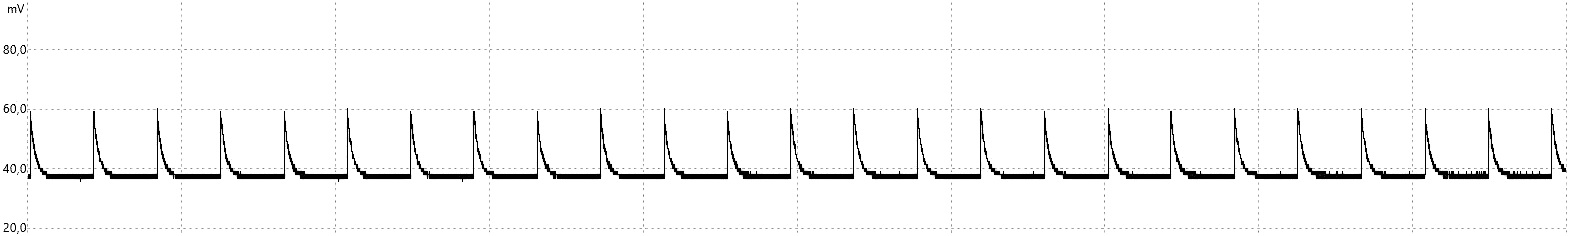
\includegraphics[width=1\linewidth]{res/idle.jpg}
	\caption{Wearable im Schlafmodus bei Batteriespannung}
	\label{fig:curSleep}
\end{figure}
\begin{figure}[!hbtp]
	\centering
	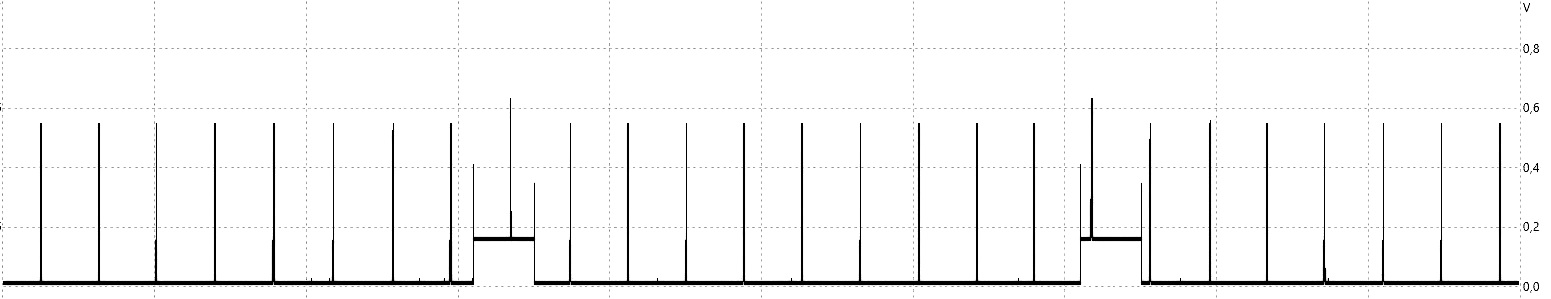
\includegraphics[width=1\linewidth]{res/wearNetzAdv.jpg}
	\caption{Advertising vom Wearable bei Netzteilspannung}
	\label{fig:curNetz}
\end{figure}
\begin{figure}[!hbtp]
	\centering
	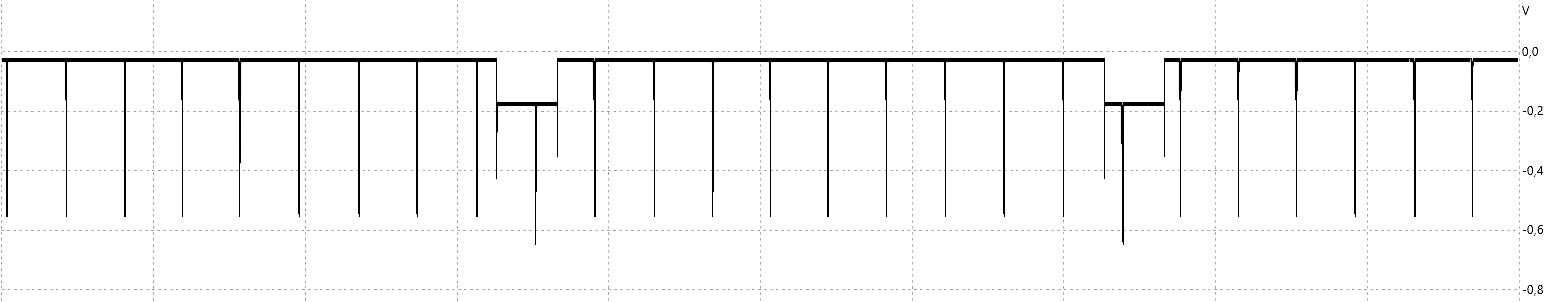
\includegraphics[width=1\linewidth]{res/wearCrAdv.jpg}
	\caption{Advertising vom Wearable bei Batteriespannung}
	\label{fig:curCr}
\end{figure}
\begin{figure}[!hbtp]
	\centering
	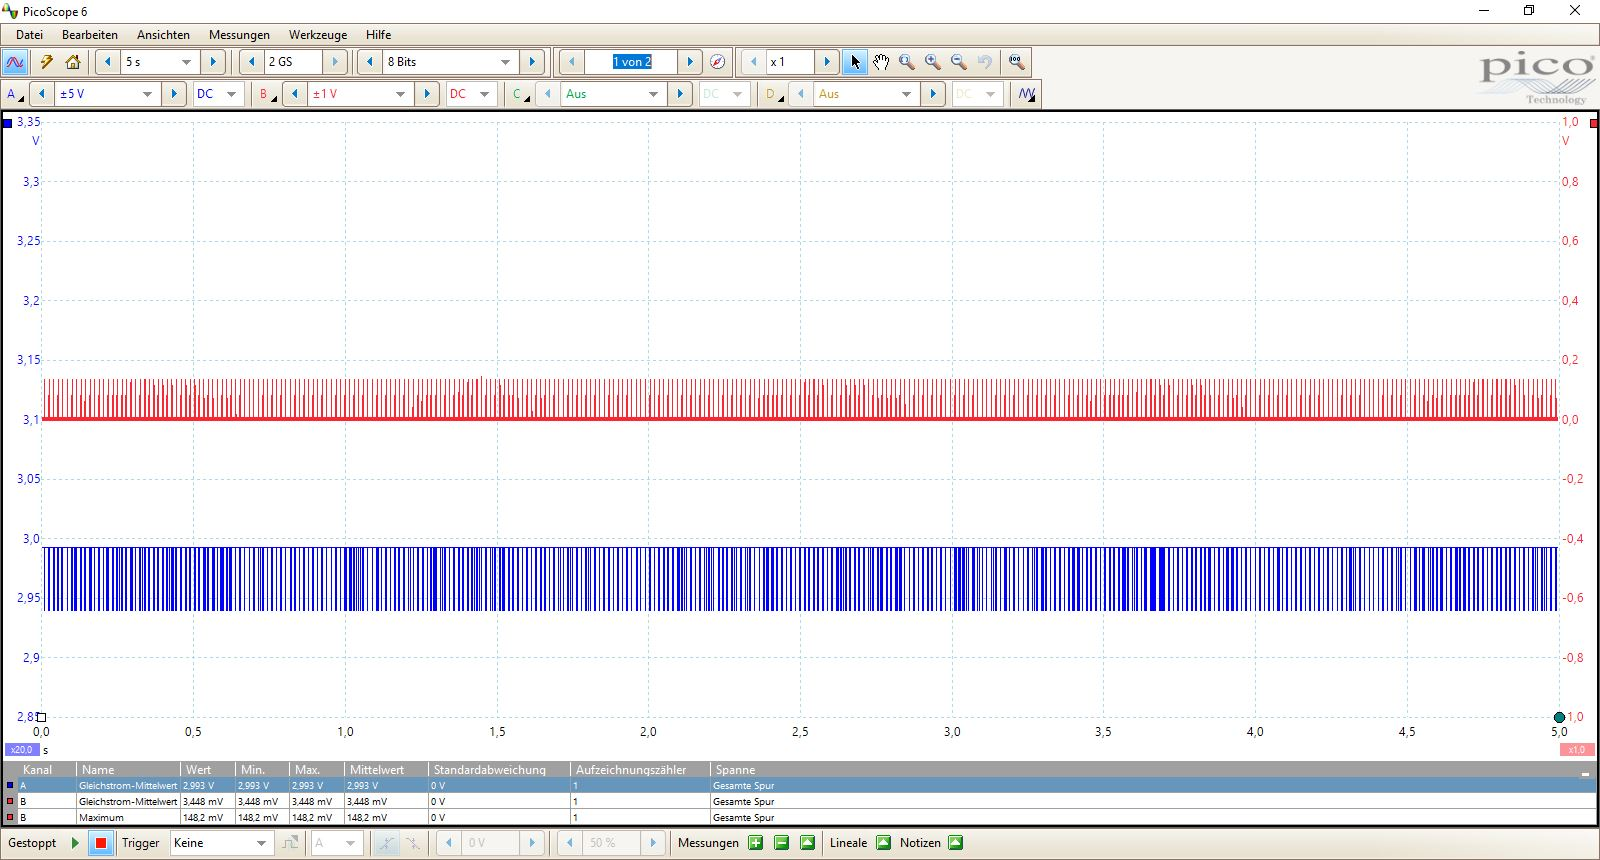
\includegraphics[width=1\linewidth]{res/wearNetz0hz.jpg}
	\caption{Verbunden mit High CI und 0 Hz bei Netzteilspannung}
	\label{fig:curHiNetz}
\end{figure}
\begin{figure}[!hbtp]
	\centering
	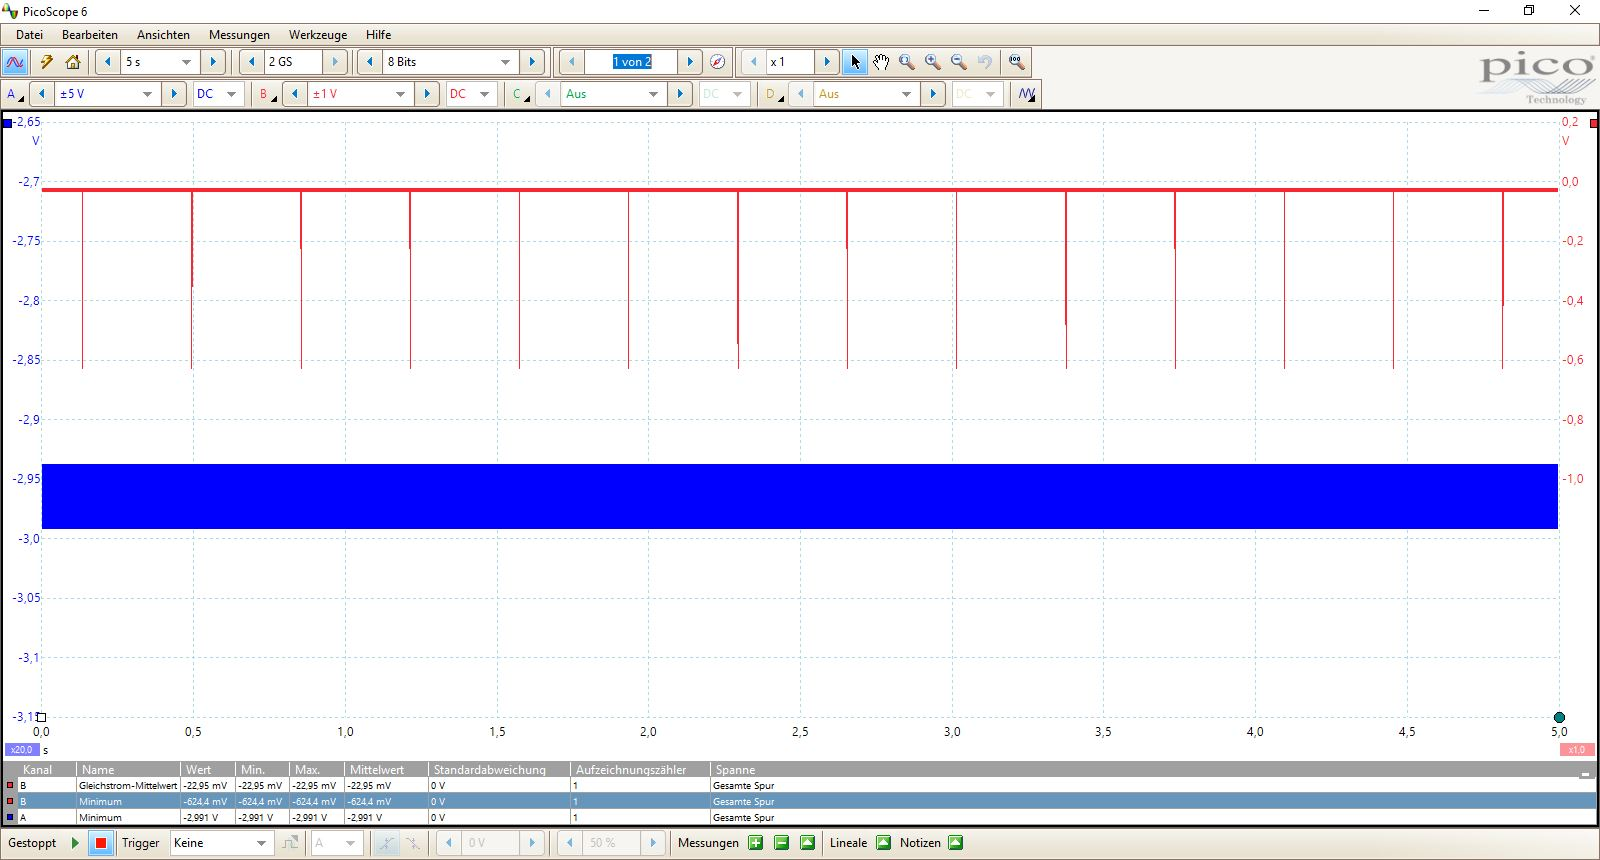
\includegraphics[width=1\linewidth]{res/ciLo0.jpg}
	\caption{Verbunden mit Low CI und 0 Hz bei Batteriespannung}
	\label{fig:curLo}
\end{figure}
\begin{figure}[!hbtp]
	\centering
	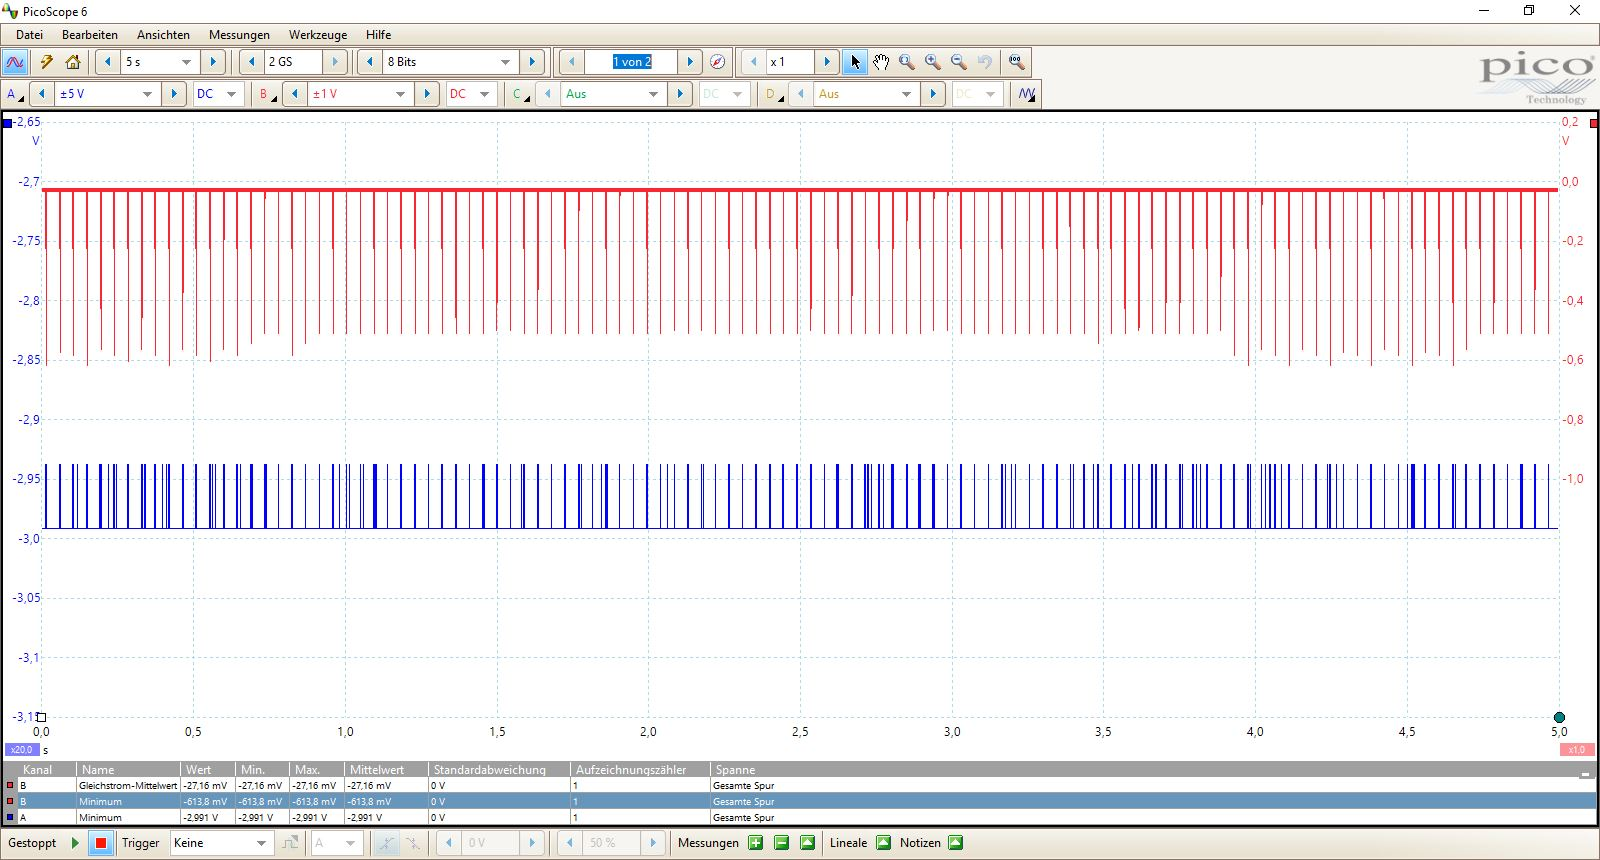
\includegraphics[width=1\linewidth]{res/ciMi0.jpg}
	\caption{Verbunden mit Balance CI und 0 Hz bei Batteriespannung}
	\label{fig:curMi}
\end{figure}
\begin{figure}[!hbtp]
	\centering
	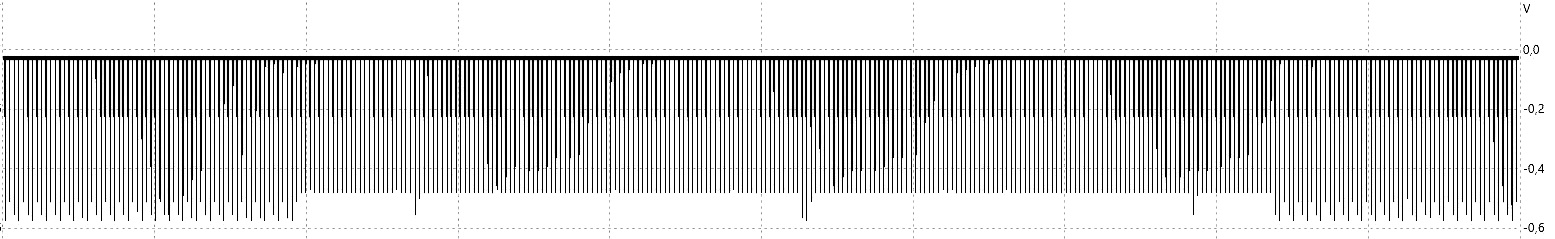
\includegraphics[width=1\linewidth]{res/ciHi0.jpg}
	\caption{Verbunden mit High CI und 0 Hz bei Batteriespannung}
	\label{fig:curHi}
\end{figure}
\begin{figure}[!hbtp]
	\centering
	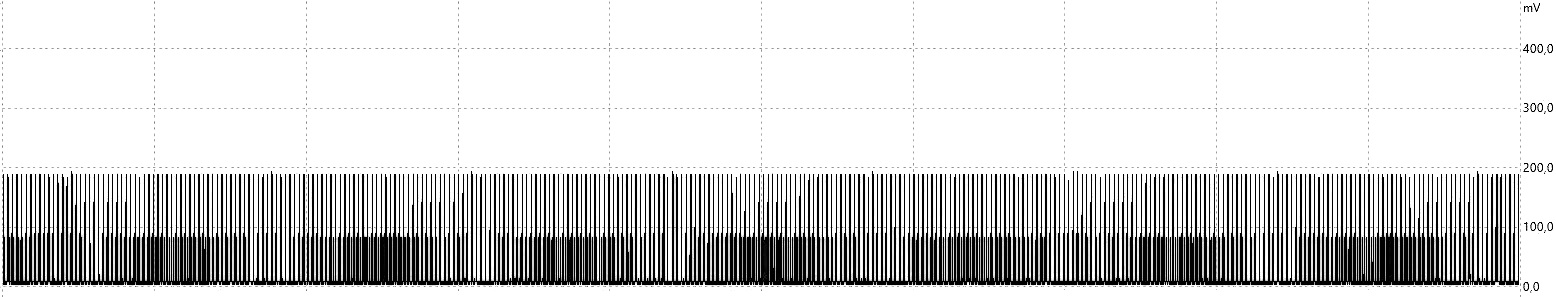
\includegraphics[width=1\linewidth]{res/wearNetzteil200hz.jpg}
	\caption{Verbunden mit High CI und 200 Hz bei Netzteilspannung}
	\label{fig:cur200}
\end{figure}

\section{Auswertung}
Zunächst ist zu beachten, dass der Ausschlag der Spannungen in den Abbildungen teilweise negativ ist.
Es hat keinerlei Auswirkungen auf die Daten und ist durch die Messweise bedingt.
Ein Abschnitt auf der X-Achse sind 0.5 Sekunden, sodass eine komplette Abbildung 5 Sekunden darstellt.
Eine Frequenz von 0 Hz bedeutet, dass die IMU keine Daten erfasst.

\subsection{Nur Stromaufnahme als Metrik?}
Vergleicht man Abbildung \ref{fig:curNetz} und Abbildung \ref{fig:curCr}, stellt man fest, dass sich die Verlaufskurven bei Batterie- und Netzspannung nicht unterscheiden.
Es sind regelmäßige Spitzen zu erkennen in denen das Wearable am Advertisen ist.
Die zusätzliche Stromaufnahme durch die blinkende LED ist beobachtbar.\\
Vergleicht man den \underline{Strom} 'Wearable LSM6DSL 200 Hz' (Tabelle \ref{tab:test1}) mit '200Hz' (Tabelle \ref{tab:test5}), stellt man einen Anstieg der Stromaufnahme von 8.51 \% bei Batteriebetrieb fest.\\
In Tabelle \ref{tab:test1} wurde mit einem 10 Ohm Widerstand gemessen, wohingegen in Tabelle \ref{tab:test5} mit 47 Ohm gemessen wurde.
Während die Spannungsquellen beide etwa 3 Volt liefern, fällt eine unterschiedliche Spannung an den Widerständen ab.
Vergleicht man den \underline{Leistungsverbrauch}, misst man immer noch einen Unterschied von 5.4 \%.\\
Werden die Werte 'Wearable LSM6DSL 0 Hz' (Tabelle \ref{tab:test1}) und 'High 0Hz' (Tabelle \ref{tab:test4}) verglichen, sind die Unterschiede noch höher.
Es handelt sich nicht wie zunächst angenommen um eine falsche Einstellung.
Abbildung \ref{fig:curHiNetz} zeigt die zugehörige Aufnahme, die dem Muster von Abbildung \ref{fig:curHi} entspricht.
Beim Batteriebetrieb ist die Stromaufnahme 120 \% und die Leistungsaufnahme 133 \% so hoch.\\\\
Während in den Datenblättern der Komponenten die Stromaufnahme bei einer bestimmten Spannung spezifiziert ist \cite{datasheet_lsm6dsl} \cite{datasheet_nrf52832}, ist die Spannung am Testobjekt bei der eingesetzten Messmethode abhängig von der Stromaufnahme.
Die Stromberechnungen mit stark unterschiedlichen Spannungsabfällen sind nicht direkt miteinander vergleichbar.
Trotzdem sind die Berechnungen für das Wearable gültig, da die Spannungen am Testobjekt über 2 Volt liegen und die Knopfzelle unter 2 Volt als leer gilt.
Es lässt sich stattdessen die Leistungsaufnahme vergleichen.
Hierbei muss beachtet werden, dass das Testobjekt bei unterschiedlichen Spannungen unterschiedlich effektiv arbeiten kann.\\
Die Stromaufnahme ist trotzdem wichtig, da die Batterien bei höherem Strom eine geringere Kapazität aufweisen.
So hat die CR2450 weniger als 600 mAh Kapazität, wenn weniger als 5.5 kOhm anliegen.
Diese Grenze ist bei 2 Volt mit 364 $\mu$A erreicht. \cite{datasheet_ds6450}

\subsection{Leistungs- und Stromeinfluss der Parameter}
Im Test mit dem Netzteil wurde eine MTU-Größe von 23 Byte gewählt.
Beim Test von der Batterie wurde sie auf 35 Byte erhöht.
Betrachtet man Tabelle \ref{tab:test2}, so stellt man fest, dass die Größe des TX-Buffers und die Größe der MTU in der Leistungsaufnahme höchstens einen Unterschied von 0.78 \% ausmachen.
Deshalb kann davon ausgegangen werden, dass sie die Leistungsaufnahme nicht beeinflussen.\\
Tabelle \ref{tab:test1} kann man entnehmen, dass der Prototyp mit LSM6DSL 20 \% mehr Strom und Leistung verbraucht als das Wearable bei 200 Hz.
Bei 0 Hz sind es 186 \% in der Strom- und 202 \% mehr in der Leistungsaufnahme.\\
Der Unterschied zwischen BMI160 und LSM6DSL ist vernachlässigbar, wenn die Sensoren keine Daten aufnehmen.\\
Bei 200 Hz verbraucht der BMI160 zwischen 18 und 19 \% mehr Strom und Leistung.
Tabelle \ref{tab:test3} beweist, dass die kleinstmögliche SPI-Frequenz 63 \% mehr Strom und 70 \% mehr Leistung als die Höchstmögliche verbraucht.
Die mittlere Frequenz befindet sich dazwischen, allerdings ist der Vorteil von 125 kHz zu 1 MHz stärker als von 1 MHz zu 8 MHz zu wechseln.\\
Tabelle \ref{tab:test4} sagt aus, dass eine Erhöhung des Connection Interval von Low auf Balance die Strom- und Leistungsaufnahme um 20 \% erhöht.
Die Erhöhung von Balance zu High beträgt 34 \%.
In den Abbildungen \ref{fig:curLo} bis \ref{fig:curHi} sieht man die Erhöhung der Anzahl der Spitzen proportional zum Connection Interval.\\
Tabelle \ref{tab:test5} zeigt, dass eine höhere Sensordatenrate auch eine höhere Aufnahme bedeutet.
Während aber eine Erhöhung von 25 Hz auf 50 Hz nur einen Zuwachs von unter 7 \% bedeutet, erhöht sich der Strom bei einem Wechsel von 400 Hz auf 800 Hz um 52 \% und die Leistung um 58 \%.\\
Abbildung \ref{fig:curSleep} ist die Stromaufnahme während des Schalfmodus der MCU.
Es sind regelmäßig Spitzen von etwa 5 $mu$A zu sehen.
Sie kommen daher, dass die MCU einen internen Spannungswandler besitzt.
Wenn der benötigte Strom gering ist, wird der Spannungswandler in Intervallen betrieben und lädt dabei einen Kondensator auf, von dem die MCU ihre Leistung beziehen kann \cite{site_refreshMode}.
Entgegen der Datenblätter von MCU und IMU nutzt das Wearable 1.537 $\mu$A statt $3.3 \mu{}A = 0.3 \mu{}A + 3 \mu{}A$ \cite{datasheet_lsm6dsl} \cite{datasheet_nrf52832}.\\
Mit der Leistungsaufnahme von 0.004 mW im Schlafmodus sollte das Wearable 53 Jahre bei einer Batteriekapazität von 620 mAh laufen.
Wird es allerdings genutzt, ist die geringste Stromaufnahme bei 25 Hz Sensordatenrate, Low Connection Interval und 8 MHz SPI-Frequenz mit etwa 1 mA zu erwarten.
Das entspricht 2 - 3 kOhm bei 2 - 3 Volt Spannung.
Während die CR2450 bei 3 kOhm weniger als 90 \% der Kapazität besitzt und für 2 kOhm nicht spezifiziert ist \cite{datasheet_ds6450}, behält die CR2032 bei dem Widerstand noch etwa die gesamte Kapazität \cite{datasheet_ds6032}.
Bei 550 mAh sollte sich die CR2450 bei 1 mA und 3 kOhm etwa 23 Tage betreiben lassen.\\
Um auszuschließen, dass sich die Batterie von Varta nicht als Referenzmodell eignet, wurde nach einem anderen Modell gesucht, dass sich besonders für hohe Ströme eignet.
Die Murata CR2450R werden explizit als ``High Drain lithium coin batteries'' \cite{site_murataCr2450r} vermarktet.
Sie haben nur eine Kapazität von 500 mAh aber die Kapazität ist bis 10 mA angegeben und der Spitzenstrom darf 50 mA betragen.
Es wird empfohlen sie unter 3 mA zu betreiben, wo sie noch etwa 450 mAh bereitstellen kann.
Das ergibt eine Laufzeit von mehr als 6 Tagen. \cite{site_murataCr2450r}\\
Damit lässt sich das Wearable mit 200 Hz Sensordatenrate betreiben (vgl. '200Hz' in Tabelle \ref{tab:test5}).
Eine Sensordatenrate von 400 Hz verbraucht selbst bei höherer SPI-Frequenz zu viel Strom (vgl. '8MHz' in Tabelle \ref{tab:test3}).
In dem Test hatte das Wearable durchschnittlich 2.871 V zur Verfügung.
Sinkt die Spannung weiter, sollte die Stromaufnahme noch höher sein.\\
Wird die Hochstrom-CR2450 mit der CR2032 der selben Modellreihe verglichen, hat die CR2450 bei 3 mA die 2.5-fache Kapazität \cite{site_murataCr2032r}.
Dagegen hat der vorherige Vergleich in Abschnitt \ref{ch:aimEval} die 2.7-fache Kapazität ergeben.
Das Volumen beträgt weiterhin das 2.34-fache bei der CR2450.

\subsection{Standardabweichung der ankommenden Datenrate}
Bei allen Einstellungen ist durchschnittlich die in der IMU eingestellte Datenrate beim Smartphone angekommen.
Die Standardabweichung hat sich allerdings bei den Einstellungen unterschieden.
Für die Standardabweichung ist ein Intervall angegeben, da die ausgegebenen Werte um etwa 0.5 Hz schwankten.
Dementsprechend muss eine hohe Ungenauigkeit berücksichtigt werden.\\
In Tabelle \ref{tab:test2} ist die Standardabweichung um mindestens 1 Hz höher wenn der Algorithmus nicht genutzt wird.
Die Größen des TX-Buffers 1 und 50 weisen keine nachweisbaren Unterschiede auf.
Die größte Einstellung des TX-Buffers bei aktiviertem Algorithmus hat eine 2 Hz geringe Standardabweichung.\\
Tabelle \ref{tab:test3} zeigt eine 4 Hz höhere Standardabweichung bei 125 kHz SPI-Frequenz, gegenüber höheren Frequenzen.\\
Tabelle \ref{tab:test4} zeigt, dass sich die Standardabweichung mit zunehmendem Connection Interval um bis zu 3 Hz verbessert.
